\chapter{LITERATURE REVIEW}
\label{chapter:literature_review}


\section{Modeling Paradigms}

\subsection{Event-Flow Graphs}
\subsection{Transition-Based Models}
\subsection{Data-Flow Models}

\section{Tool Review}
\subsection{Spec Explorer}
\par
Spec Explorer \cite{SpecExplorer_Description} is a \acrshort{mbt} tool which has been developed by Microsoft Research between 2004 and 2010. It has been used within for testing within Microsoft on a daily basis. Spec Explorer is in form of Add-On to Microsoft Visual Studio \acrshort{ide}, but now it seems to be not supported any more, as it is not compatible to versions of Visual Studio \acrshort{ide} released after 2012.
\par
Models in Spec Explorer are written as programming code. For writing models any .NET language can be used, such as C\#. Written models contain a set of rules which interact with a defined state. Cord is a scripting language, which is used for combining model programs. This gives the description to test generation algorithms in which ways model programs can be explored. Model program together with Cord scripts creates behavioral model of \acrlong{aut}.

\par
Spec Explorer applies state-based modeling paradigm and created behavioral models are represented in form of \acrshort{fsm}. It applies different coverage criteria for test generation, such as data coverage of parameter values, coverage of state space or coverage of all transitions through model. Test generation can be off-line as well as applied together with execution on-line.

\par
Spec Explorer also has model viewer module in which user can see the visual representation of created behavioral. It is shown in the figure below.

\begin{figure} [htbp!]
	\centering
					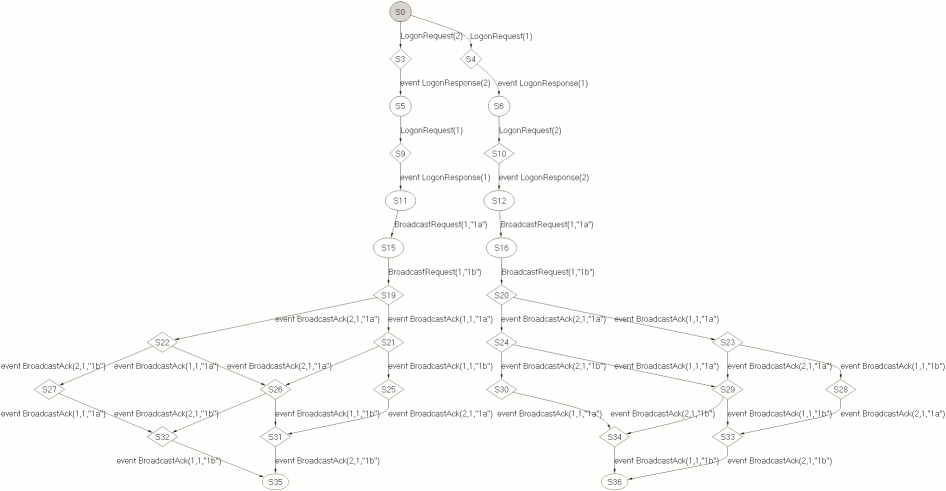
\includegraphics[width=1\textwidth]{figures/Model_View_In_SpecExplorer.png}
					\caption{\label{Fig:Model_View_In_SpecExplorer} Visual Representation of Model in Spec Explorer \cite{SpecExplorer_ModelView}}
\end{figure}

\par
When created \acrshort{fsm} has extensively big or even infinite state space, technique called Slicing is used for generation of smaller subset of the full behavior models which are more suitable for testing.

\par
One of the examples for usage of Spec Explorer in practice was provided by Jose L. Silva et. al. \cite{Silva_SpecExplorer} where they applied it together with ConcurTaskTrees. They created task models using ConcurTaskTrees notation
and used tool TERESA for generation \acrshort{fsm} from it. For creating Spec\# model, Generated \acrshort{fsm} was given as input to the tool called TOM (Task to Oracle Mapping tool) which was developed in scope of that research. The last step was generation of tests from Spec\# models using Spec Explorer and mapping the generated tests to a test driver which executed test against \acrshort{aut}.

\subsection{NModel}
\par
NModel \cite{NModel_Description} \cite{NModel_Description2} is a modeling framework created on experiences of Spec Explorer. Unlike the Spec Explorer, which uses separate compiler for compiling Spec\# models, NModel uses the standard .NET v2.0 compiler. Modeling with NModel requires coding knowledge as models need to be written using C\#.

\par
Based on the writen model, NModel generates \acrshort{fsm} or \acrshort{efsm} which can be later traversed with different coverage criteria passed to modules responsible for test generation.

\par
NModel consists of following multiple artifacts. The NModel library is bringing with it attributes and data types for writing models. It can be referenced to any type of C\# project just like any other library. Model Program Viewer (mpv) shown in figure below and Model Program to Dot (mp2dot are modules responsible for visualization and analysis of the created model. Offline Test Generator (otg) provides opportunity generate test suite off-line. Conformance Tester (ct) module can be used of both, off-line as well as on-line \acrshort{mbt}.

\begin{figure} [htbp!]
	\centering
					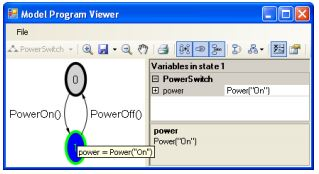
\includegraphics[width=0.5\textwidth]{figures/NModel_mpv.JPG}
					\caption{\label{Fig:NModel_mpv} Model Program Viewer of NModel}
\end{figure}


\par
We encountered usage of NModel couple of times during the literature review. In one of them Chinnapongse et. al. \cite{Chinnapongse_NModel} used NModel for testing \acrshort{gui} of The Armed Forces Health Longitudinal Tracking Application–Mobile (AHLTA-Mobile). The application is based on Windows Phone platform and has multiple modules. In scope of research they tested Military Acute Concussion Evaluation (MACE) module which consisted of 8 different GUI Screens. They started with creating mental model of the application, which was later coded in C\#. The resulting artifact was \acrshort{efsm} which was used to generate tests off-line. The last part was executing the generated tests against the MACE module.
\par
Another encountered user of NModel was Gabriel Kolawole \cite{Kolawole_NModel} who tested \acrshort{gui} and functinality of Moodle Mobile Application in scope of his master thesis. 

\subsection{MobiGUITAR}
\par
MobiGUITAR \cite{MobiGUITAR} was introduced with collaboration of researchers from University of Naples Federico II and University of Maryland. Their previous project, GUI ripping \cite{GUIripping}, was created for desktop applications and was based on \acrshort{efg}, but as mobile applications are very state sensitive, they decided to change approach and made MobiGUITAR base on \acrshort{fsm}. Currently MobiGUITAR is limited to only android platform.

\par
Testing process with MobiGUITAR is divided into three parts: ripping, generation and execution. Ripping dynamically explores application and creates \acrshort{fsm} with application states and events. Generated \acrshort{fsm} looks like figure below.

\begin{figure} [htbp!]
	\centering
					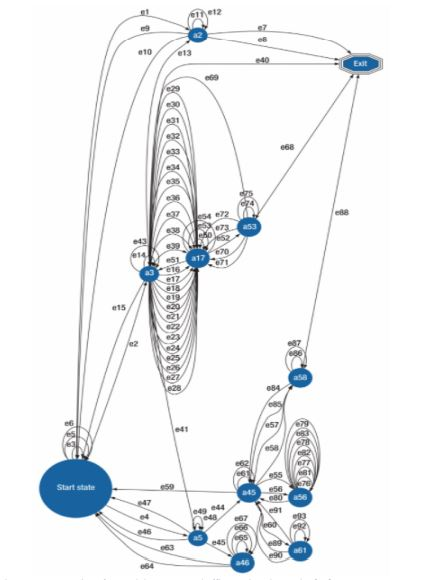
\includegraphics[width=0.5\textwidth]{figures/mobiguitar.JPG}
					\caption{\label{Fig:MobiGuitar} The abstract state machine for AardDict\cite{MobiGUITAR}}
\end{figure}

Generation uses \acrshort{fsm} created and also coverage criteria such as pair-wise edge coverage to generate test cases. This means that all pairs of adjacent edges need to be taken together.
Execution applies JUnit framework for testing \acrshort{aut} and returning the results to a tester. Basically, with these 3 parts together MobiGUITAR automates not only test generation and execution, but also modeling process itself which gives it advantage against other \acrshort{mbt} tools.

\par
Inability of functional testing is the main disadvantage which MobiGUITAR has. It is mentioned in \cite{MobiGUITAR} that, tester can enhance the JUnit tests with assertions for detecting functional errors, but that will not be easy task, because assertion of states might strongly depend with which event this state is reached. Besides that, after firing same event from same state, depending on background variables landing state might be different. For applications such as Brainloop Secure Client, verifying that functional part works as designed has the highest priority while testing that \acrshort{gui} is displayed correctly has a bit lower priority. MobiGUITAR would be very useful for example for verification of \acrshort{gui} correctness, or verification that there are no crashes and unhandled exceptions after transitions from one state to another. But in our case, that is definately not enough.

\subsection{Graphwalker}
\subsection{USE}
\subsection{Alloy Analyzer}
\subsection{ZLive}
\subsection{ProZ}
\subsection{Agile Requirements Designer from CA Technologies}

\section{Justification of Decision}